\chapter{Análisis del Software}

\section{Entorno de proyecto}
Los primeros componentes que se describirán son los relacionados con el entorno
del proyecto, que son aquellos factores del contexto que incluyen recursos
necesarios, restricciones, y cualquier otro elemento del proyecto que debe ser
tomado en cuenta para la evaluación.

\subsection{Fuentes de Información}
Para evaluar los componentes definidos en el proyecto, se encontraron
y recurrirán a las siguientes fuentes de información respecto al producto:

\begin{description}
\item [Centro de Ayuda] \emph{Salesforce} ofrece un amplio conjunto de
documentación, información general, preguntas frecuentes, y contacto con el
servicio de asistencia técnica desde su sitio de ayuda
(\emph{https://help.salesforce.com/}).

Estos recursos serán útiles para conocer los clamores de los usuarios, las
características criticas del producto, y las estrategias del fabricante hacia
sus clientes.

\item [Centro de Desarrollo] \emph{Salesforce} también posee un sitio web
específicamente para compartir recursos de desarrollo sobre la plataforma
(\emph{https://developer.salesforce.com/}).

Este sitio se podrá aprovechar para consultar las referencias a las API del
servicio, conocer las posibilidades que proveen los componentes y como pueden
aprovecharse desde la perspectiva del desarrollador.

\item [Recursos para administradores] Sitio web enfocado a ofrecer experiencias,
vídeos, herramientas, y un sin fin de recursos orientados a usuarios con un rol
administrativo de recursos sobre la plataforma
(\emph{https://admin.salesforce.com/resources}).

Este sitio será útil para entender las diferencias existentes entre la
funcionalidad provista a un usuario normal y a otro administrador, además de
conocer los permisos y roles de usuario en profundo.

\item [Comunidad \emph{Trailblazer}] Sitio web enfocado a conectar a miembros de
la comunidad \emph{Salesforce}, para compartir experiencias, aprender, y proveer
de nuevas ideas sobre la utilización del servicio
(\emph{https://success.salesforce.com/}).

Este sitio también sirve como fuente de clamores de los usuarios,
funcionalidades criticas, y errores comunes encontrados en el servicio.

\end{description}

\subsection{\emph{Salesforce}}
\emph{Salesforce} cuenta con múltiples ediciones que comparten una apariencia,
pero varían según la funcionalidad y los costos del servicio. Según la
documentación del fabricante algunos clientes comienzan con una edición básica y
actualizan a una edición más rica en características a medida que evolucionan
los requisitos empresariales.

En el cuadro \ref{ediciones} se describen las ediciones disponibles con las que
cuenta el servicio actualmente\footnote{Información extraída y disponible en:
https://help.salesforce.com/articleView?id=overview\_edition.htm}, cabe comentar
que la evaluación se realizará sobre la versión \emph{Developer} debido a que
está es la que requiere para su utilización, la menor cantidad de restricciones
de parte del fabricante.

\begin{table}[H]
\centering
\begin{tabular}{|l|p{12.0cm}|}
\hline
\footnotesize{\textbf{Edición}} & \footnotesize{\textbf{Descripción}} \\
\hline
\footnotesize{\emph{Essentials}} & \footnotesize{Diseñado para pequeños negocios
para empezar a trabajar con un sistema de CRM de forma rápida. Incluye
presentaciones interactivas y un asistente de configuración para comenzar, una
interfaz de usuario fácil de utilizar y herramientas de administración para
personalizar su implementación conforme crece.} \\
\footnotesize{\emph{Professional}} & \footnotesize{Diseñado para negocios que
requieren la funcionalidad completa de CRM. Incluye herramientas de
personalización, integración y administración directas y fáciles de usar para
facilitar cualquier implementación de pequeño y mediano tamaño.} \\
\footnotesize{\emph{Enterprise}} & \footnotesize{Cumple las necesidades
comerciales grandes y complejas. Proporciona herramientas avanzadas de
personalización y administración, además de todas las funcionalidades
disponibles en Professional Edition, que pueden admitir implementaciones a gran
escala. Enterprise Edition también incluye acceso a las API de Salesforce para
que pueda integrar fácilmente sistemas de gestión interna.} \\
\footnotesize{\emph{Unlimited}} & \footnotesize{Proporciona nuevos niveles de
flexibilidad de plataforma para gestionar y compartir toda su información según
demanda. Incluye todas las funcionalidades de Enterprise Edition además de
Premier Support, acceso móvil completo, aplicaciones personalizadas sin límite,
límites de almacenamiento ampliados y otras funciones.} \\
\footnotesize{\emph{Developer}} & \footnotesize{Proporciona acceso a las API y
la plataforma Lightning. Permite a los desarrolladores ampliar Salesforce,
integrarlo con otras aplicaciones y desarrollar nuevas herramientas y
aplicaciones. Developer Edition ofrece además acceso a muchas de las funciones
disponibles en Enterprise Edition.} \\
\hline
\end{tabular}
\caption{Ediciones actualmente disponibles de \emph{Sales Cloud}.}
\label{ediciones}
\end{table}

Otra característica actual de \emph{Salesforce} es que cuenta con dos interfaces
web diferentes: la antigua conocida como: \emph{Salesforce Classic}, y la nueva
incluida desde 2015 denominada: \emph{Salesforce Lightning}; que tiene como
objetivo principal la unificación del comportamiento y la apariencia a través de
todo el servicio sea cual sea el dispositivo que el cliente
utilice \cite{McCarthy}.

Se evaluarán las funcionalidades de los módulos sobre el navegador cuya
participación en el mercado es la mayor, en este caso: \emph{Google Chrome}
como puede verse en la figura \ref{software}.

\begin{figure}[H]
\centering
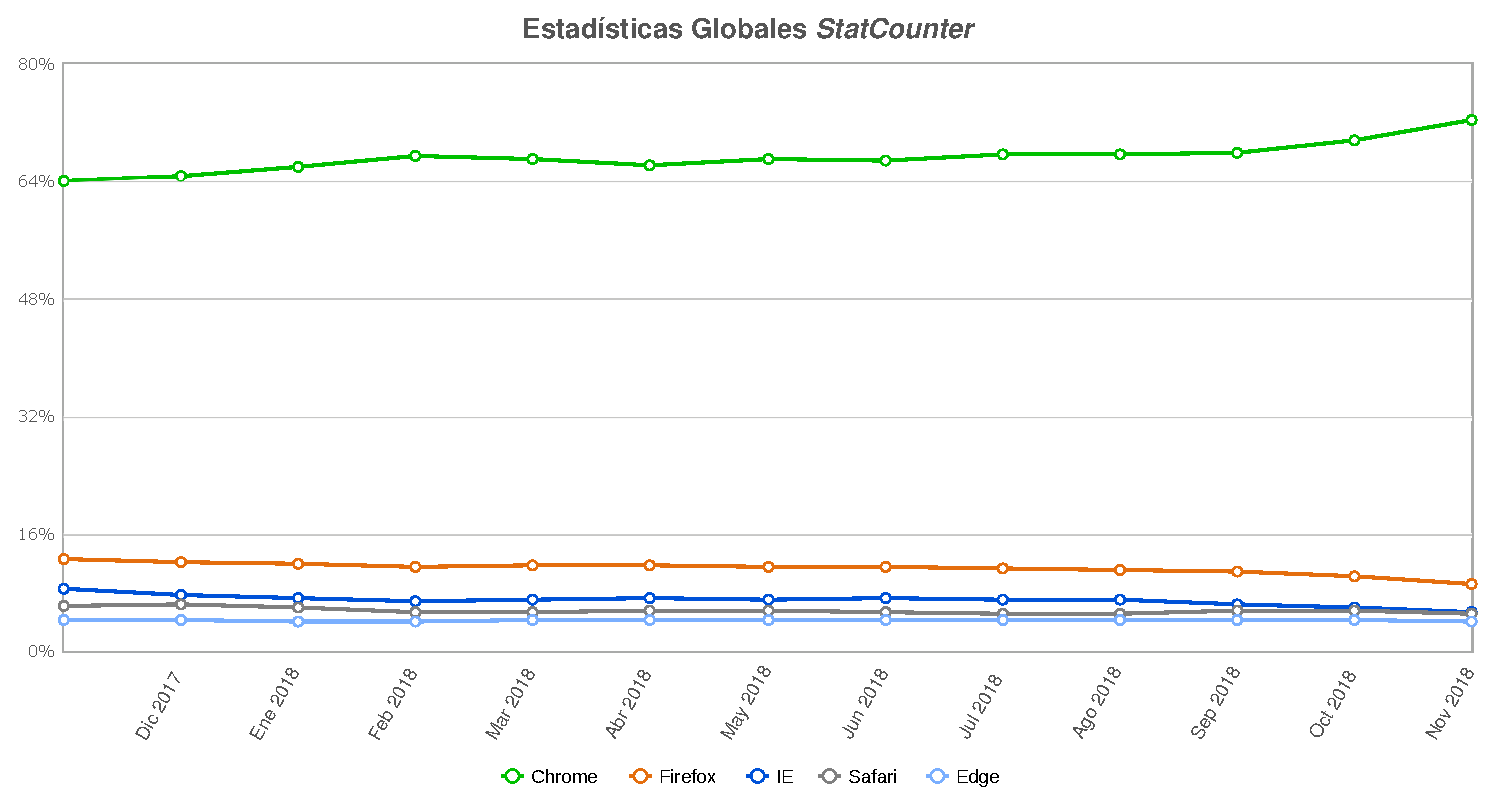
\includegraphics[width=1.0\textwidth]{graphics/compatibilidad.eps}
\caption{Participación de mercado de los navegadores hasta Noviembre del 2018.}
\label{software}
\end{figure}

Adicionalmente al uso del navegador \emph{Google Chrome} serán necesarios
otros navegadores para realizar la evaluación de compatibilidad sobre
vistas especificas del sistema, para este fin se consultó la información
disponible en la pagina de soporte provista por el fabricante, la cual como
puede verse en el cuadro \ref{soporte_navegadores}, nos dice que se soportan
cinco navegadores diferentes bajo condiciones de limitación conocidas por el
fabricante\footnote{Información extraída y disponible en:
https://help.salesforce.com/articleView?id=getstart\_browsers\_sfx.htm}.

\begin{table}[H]
\centering
\begin{tabular}{|p{6.0cm}|p{2.5cm}|p{1.4cm}|p{1.3cm}|p{1.3cm}|p{1.0cm}|}
\hline
& \footnotesize{\textbf{Microsoft Internet Explorer}}
& \footnotesize{\textbf{Microsoft Edge}}
& \footnotesize{\textbf{Google Chrome}}
& \footnotesize{\textbf{Mozilla Firefox}}
& \footnotesize{\textbf{Apple Safari}} \\
\hline
\footnotesize{Lightning Experience}
& \footnotesize{IE11 (EOL Diciembre 31, 2020)}
& \footnotesize{Ultima versión}
& \footnotesize{Ultima versión}
& \footnotesize{Ultima versión}
& \footnotesize{11.x+} \\
\footnotesize{Lightning Communities}
& \footnotesize{IE11 (EOL Diciembre 31, 2020)}
& \footnotesize{Ultima versión}
& \footnotesize{Ultima versión}
& \footnotesize{Ultima versión}
& \footnotesize{11.x+} \\
\footnotesize{¿Consideraciones especiales de configuración?}
& \footnotesize{No}
& \footnotesize{No}
& \footnotesize{No}
& \footnotesize{No}
& \footnotesize{No} \\
\footnotesize{Limitaciones conocidas}
& \footnotesize{Sí}
& \footnotesize{Si}
& \footnotesize{No}
& \footnotesize{Si}
& \footnotesize{Si} \\
\hline
\end{tabular}
\caption{Lista de compatibilidad provista por \emph{Salesforce}.}
\label{soporte_navegadores}
\end{table}

\section{Elementos del producto}
Dentro del alcance de la evaluación se encuentran los componentes de productos
y listas de precios, las funcionalidades que comprenden estos se detallan en
esta sección, desde múltiples perspectivas de análisis.

Como se mencionó anteriormente en la sección de equipamiento, se consideró la
interfaz \emph{Lightning Experience}, como único objetivo de la evaluación. La
versión \emph{Lightning Experience} esta disponible para las siguientes
ediciones del producto: \emph{Essentials}, \emph{Group}, \emph{Professional},
\emph{Enterprise}, \emph{Performance}, \emph{Unlimited}, y \emph{Developer}.

\subsection{Productos}
El Producto para el software a evaluar, representa uno de los componentes
fundamentales y claves para el éxito, por ende es importante evaluarlo
desde múltiples facetas; la primera de estas es la funcionalidad provista por
las interfaces de este modulo. En la figura \ref{productos} pueden verse estas
funcionalidades, clasificadas desde la perspectiva de la interfaz de usuario.

Entre las funcionalidades que pueden apreciarse, están las operaciones comunes
de creación, búsqueda, visualización, modificación, y eliminación de productos,
se omitieron las funcionalidades de controles de vista de lista, para que
todo este componente pueda ser tratado de manera separada. También pueden
observarse funciones relacionadas a registrar precios estándar y precios para
una lista de precios determinada.

En la figura \ref{productos_vistas}, se aprecian las diferentes vistas que
comprenden el modulo, se resalto con color amarillo aquellas vistas que son de
tipo formulario, mientras que se resalto con color verde aquellas que son de
tipo confirmación de acción.

Además de las funcionalidades y vistas antes mencionadas, también se analizo el
comportamiento de los formularios que provee el modulo, los cuales se presentan
en la figura \ref{productos_formularios}.

\begin{figure}[H]
\centering
\begin{tikzpicture}[
    grow via three points={one child at (0.5,-0.7) and
    two children at (0.5,-0.7) and (0.5,-1.4)},
    edge from parent path={(\tikzparentnode.south) |- (\tikzchildnode.west)}]
    \node {Productos}
        child { node {Nuevo}}
        child { node {Buscar: Producto}}
        child { node {Controles de Vista de Lista}
            child { node {\ldots}}
        }
        child [missing] {}
        child { node {Mostrar como}}
        child { node {Actualizar}}
        child { node {Filtrar por: Vista de Lista}}
        child { node {Modificar Lista}}
        child { node {Lista de Productos}
            child { node {Ver: Producto}
                child { node {Modificar}}
                child { node {Eliminar}}
                child { node {Duplicar}}
                child { node {Relacionado}
                    child { node {Agregar precio estándar}}
                    child { node {Agregar a lista de precios}}
                    child { node {Ver: Lista de precios}}
                    child { node {Modificar: Lista de precios}}
                    child { node {Eliminar: Lista de precios}}
                    child { node {Ver todos}
                        child { node {Actualizar}}
                    }
                }
                child [missing] {}
                child [missing] {}
                child [missing] {}
                child [missing] {}
                child [missing] {}
                child [missing] {}
                child [missing] {}
                child { node {Detalles}}
            }
            child [missing] {}
            child [missing] {}
            child [missing] {}
            child [missing] {}
            child [missing] {}
            child [missing] {}
            child [missing] {}
            child [missing] {}
            child [missing] {}
            child [missing] {}
            child [missing] {}
            child [missing] {}
            child { node {Modificar: Producto}}
            child { node {Eliminar: Producto}}
        };
\end{tikzpicture}
\caption{Funciones que componen el módulo de gestión de productos.}
\label{productos}
\end{figure}

\begin{figure}[H]
\centering
\begin{tikzpicture}[
    grow via three points={one child at (0.5,-0.7) and
    two children at (0.5,-0.7) and (0.5,-1.4)},
    edge from parent path={(\tikzparentnode.south) |- (\tikzchildnode.west)}]
    \node {Productos}
        child { node {Mostrar como}
            child { node {Tabla}}
            child { node {Kanban}}
        }
        child [missing] {}
        child [missing] {}
        child { node [form] {Crear Producto}}
        child { node {Filtros}}
        child { node {Producto}
            child { node [form] {Modificar: Producto}}
            child { node [confirm] {Eliminar: Producto}}
            child { node [form] {Crear Producto}}
            child { node {Detalles}}
            child { node {Relacionado}
                child { node [form] {Crear Entrada del catalogo de precios}}
                child { node [form] {Agregar a lista de precios}}
                child { node {Listas de precios}
                    child { node [form] {Modificar Entrada del catalogo de precios}}
                    child { node [confirm] {Eliminar entrada del catalogo de precios}}
                }
            }
        }
        child [missing] {}
        child [missing] {}
        child [missing] {}
        child [missing] {}
        child [missing] {}
        child [missing] {}
        child [missing] {}
        child [missing] {}
        child [missing] {}
        child [missing] {}
        child { node [form] {Modificar: Producto}}
        child { node [confirm] {Eliminar: Producto}};
\end{tikzpicture}
\caption{Vistas que componen el módulo de gestión de productos.}
\label{productos_vistas}
\end{figure}

\begin{figure}[H]
\centering
\begin{tikzpicture}[
    grow via three points={one child at (0.5,-0.7) and
    two children at (0.5,-0.7) and (0.5,-1.4)},
    edge from parent path={(\tikzparentnode.south) |- (\tikzchildnode.west)}]
    \node {Productos}
        child { node {Crear producto}
            child { node {Nombre del producto (*)}}
            child { node {Activo}}
            child { node {Código de producto}}
            child { node {Familia de productos}}
            child { node {Descripción del producto}}
        }
        child [missing] {}
        child [missing] {}
        child [missing] {}
        child [missing] {}
        child [missing] {}
        child { node {Crear entrada del catálogo de precios}
            child { node {Producto (*)}}
            child { node {Activo}}
            child { node {Lista de precios (*)}}
            child { node {Precio de la lista (*)}}
            child { node {Utilizar precio estándar}}
        }
        child [missing] {}
        child [missing] {}
        child [missing] {}
        child [missing] {}
        child [missing] {}
        child { node {Agregar a lista de precios}
            child { node {Lista de precios (*)}}
            child { node {Divisa (*)}}
        }
        child [missing] {}
        child [missing] {}
        child { node {Modificar entrada del catálogo de precios}
            child { node {Activo}}
            child { node {Precio de la lista (*)}}
            child { node {Utilizar precio estándar}}
        };
\end{tikzpicture}
\caption{Formularios que componen el módulo de gestión de productos.}
\label{productos_formularios}
\end{figure}

\subsection{Listas de Precios}
Las Listas de Precios, tienen como objetivo, hacer que un mismo producto pueda
tener múltiples precios, dependiendo de como la organización cliente maneje sus
canales de distribución y producción. Al igual que en el modulo de productos, en
la figura \ref{listas_de_precios} pueden verse las funcionalidades clasificadas
desde la perspectiva de la interfaz de usuario, también se omitió la sección de
los controles de vista de lista.

Las funciones de Listas de Precios son muy similares a aquellas vistas en el
modulo de productos, analizado anteriormente.

En la figura \ref{listas_de_precios_vistas}, se detallan aquellas vistas
presentes en este modulo, de la misma manera se ha destacado con amarillo a
aquellas vistas que son formularios, mientras que en verde se presentan a
aquellas que representan diálogos de confirmación.

También de las funcionalidades y vistas antes mencionadas, se analizo el
comportamiento de los formularios que provee este modulo, los cuales se
presentan en la figura \ref{listas_de_precios_formularios}.

\begin{figure}[H]
\centering
\begin{tikzpicture}[
    grow via three points={one child at (0.5,-0.7) and
    two children at (0.5,-0.7) and (0.5,-1.4)},
    edge from parent path={(\tikzparentnode.south) |- (\tikzchildnode.west)}]
    \node {Listas de Precios}
        child { node {Nuevo}}
        child { node {Buscar: Lista de precios}}
        child { node {Controles de Vista de Lista}
            child { node {\ldots}}
        }
        child [missing] {}
        child { node {Mostrar como}}
        child { node {Actualizar}}
        child { node {Filtrar por: Vista de Lista}}
        child { node {Modificar Lista}}
        child { node {Lista de Listas de Precios}
            child { node {Ver: Lista de precios}
                child { node {Modificar}}
                child { node {Eliminar}}
                child { node {Duplicar}}
                child { node {Relacionado}
                    child { node {Agregar productos}}
                    child { node {Ver: Producto}}
                    child { node {Modificar: Producto}}
                    child { node {Eliminar: Producto}}
                    child { node {Ver todos}
                        child { node {Actualizar}}
                    }
                    child [missing] {}
                    child { node {Historial de lista de precios (Ver todos)}
                        child { node {Actualizar}}
                    }
                }
                child [missing] {}
                child [missing] {}
                child [missing] {}
                child [missing] {}
                child [missing] {}
                child [missing] {}
                child [missing] {}
                child [missing] {}
                child { node {Detalles}}
            }
            child [missing] {}
            child [missing] {}
            child [missing] {}
            child [missing] {}
            child [missing] {}
            child [missing] {}
            child [missing] {}
            child [missing] {}
            child [missing] {}
            child [missing] {}
            child [missing] {}
            child [missing] {}
            child [missing] {}
            child { node {Modificar: Lista de Precios}}
            child { node {Eliminar: Lista de Precios}}
        };
\end{tikzpicture}
\caption{Funciones que componen el módulo de gestión de listas de precios.}
\label{listas_de_precios}
\end{figure}

\begin{figure}[H]
\centering
\begin{tikzpicture}[
    grow via three points={one child at (0.5,-0.7) and
    two children at (0.5,-0.7) and (0.5,-1.4)},
    edge from parent path={(\tikzparentnode.south) |- (\tikzchildnode.west)}]
    \node {Listas de Precios}
        child { node {Mostrar como}
            child { node {Tabla}}
            child { node {Kanban}}
        }
        child [missing] {}
        child [missing] {}
        child { node [form] {Crear Lista de precios}}
        child { node {Filtros}}
        child { node {Lista de precios}
            child { node [form] {Modificar: Lista de Precios}}
            child { node [form] {Crear Lista de precios}}
            child { node [confirm] {Eliminar: Lista de precios}}
            child { node {Detalles}}
            child { node {Relacionado}
                child { node [form] {Agregar productos}
                    child { node [form] {Modificar Entrada del catalogo de precios}}
                }
                child [missing] {}
                child { node {Productos}
                    child { node [form] {Modificar Entrada del catalogo de precios}}
                    child { node [confirm] {Eliminar Entrada del catalogo de precios}}
                }
                child [missing] {}
                child [missing] {}
                child { node {Historial de lista de precios}}
            }
        }
        child [missing] {}
        child [missing] {}
        child [missing] {}
        child [missing] {}
        child [missing] {}
        child [missing] {}
        child [missing] {}
        child [missing] {}
        child [missing] {}
        child [missing] {}
        child [missing] {}
        child { node [form] {Modificar: Lista de Precio}}
        child { node [confirm] {Eliminar: Lista de Precio}};
\end{tikzpicture}
\caption{Vistas que componen el módulo de gestión de listas de precios.}
\label{listas_de_precios_vistas}
\end{figure}

\begin{figure}[H]
\centering
\begin{tikzpicture}[
    grow via three points={one child at (0.5,-0.7) and
    two children at (0.5,-0.7) and (0.5,-1.4)},
    edge from parent path={(\tikzparentnode.south) |- (\tikzchildnode.west)}]
    \node {Listas de Precios}
        child { node {Crear lista de precios}
            child { node {Nombre de la lista de precios (*)}}
            child { node {Activo}}
            child { node {Descripción}}
            child { node {Es lista de precios estándar}}
        }
        child [missing] {}
        child [missing] {}
        child [missing] {}
        child [missing] {}
        child { node {Agregar productos}
            child { node {Buscar entrada de catálogos de precios}
                child { node {Modificar Entrada de catálogos de precios}}
            }
        };
\end{tikzpicture}
\caption{Formularios que componen el módulo de gestión de listas de precios.}
\label{listas_de_precios_formularios}
\end{figure}

\subsection{Controles de Vista de Lista}
Los Controles de Vista de Lista son funcionalidades equivalentes entre los 
dos componentes que están siendo evaluados, por lo que se ha decidido realizar
un análisis separado de estos. En la figura \ref{vista_de_lista} puede verse
las funciones omitidas en los diagramas anteriores relativas a los controles de
vista.

En la figura \ref{vista_de_lista_vistas}, se detallan aquellas vistas
provistas por este componente, de la misma manera que en los dos módulos
anteriormente citados, aquí también se han destacado con amarillo a
aquellas vistas que son formularios, mientras que en verde se presentan a
aquellas que representan diálogos de confirmación.

También de las funcionalidades y vistas antes mencionadas, se analizo el
comportamiento de los formularios que provee este modulo, los cuales se
presentan en la figura \ref{vista_de_lista_formularios}.

\begin{figure}[H]
\centering
\begin{tikzpicture}[
    grow via three points={one child at (0.5,-0.7) and
    two children at (0.5,-0.7) and (0.5,-1.4)},
    edge from parent path={(\tikzparentnode.south) |- (\tikzchildnode.west)}]
    \node {Controles de Vista de Lista}
        child { node {Nuevo}}
        child { node {Duplicar}}
        child { node {Cambiar nombre}}
        child { node {Configuración de colaboración}
            child { node {Modificar}}
        }
        child [missing] {}
        child { node {Modificar filtros de lista}
            child { node {Ver/Modificar: Filtro}}
            child { node {Eliminar: Filtro}}
            child { node {Agregar Filtro}}
            child { node {Eliminar todos}}
            child { node {Agregar lógica de filtro}}
        }
        child [missing] {}
        child [missing] {}
        child [missing] {}
        child [missing] {}
        child [missing] {}
        child { node {Seleccionar los campos que se visualizaran}}
        child { node {Eliminar}}
        child { node {Restablecer anchuras de columna}}
        child { node {Configuración de Kanban}};
\end{tikzpicture}
\caption{Funciones que componen el módulo de gestión de vistas de lista.}
\label{vista_de_lista}
\end{figure}

\begin{figure}[H]
\centering
\begin{tikzpicture}[
    grow via three points={one child at (0.5,-0.7) and
    two children at (0.5,-0.7) and (0.5,-1.4)},
    edge from parent path={(\tikzparentnode.south) |- (\tikzchildnode.west)}]
    \node {Vista de Lista}
        child { node [form] {Nueva vista de lista}}
        child { node [form] {Duplicar vista de lista}}
        child { node [form] {Cambiar nombre}}
        child { node [form] {Configuración de colaboración}}
        child { node [form] {Seleccionar los campos que se visualizaran}}
        child { node [confirm] {Eliminar}}
        child { node [form] {Configuración de Kanban}};
\end{tikzpicture}
\caption{Vistas que componen el módulo de gestión de listas de precios.}
\label{vista_de_lista_vistas}
\end{figure}

\begin{figure}[H]
\centering
\begin{tikzpicture}[
    grow via three points={one child at (0.5,-0.7) and
    two children at (0.5,-0.7) and (0.5,-1.4)},
    edge from parent path={(\tikzparentnode.south) |- (\tikzchildnode.west)}]
    \node {Vista de lista}
        child { node {Nueva vista de lista}
            child { node {Nombre de la lista (*)}}
            child { node {List API Name (*)}}
            child { node {¿Quien ve esta vista de lista?}
                child { node {Solo yo puedo ver esta vista de lista}}
                child { node {Todos los usuarios pueden ver esta vista de lista}}
                child { node {Compartir vista de lista con grupos de usuarios}}
            }
        }
        child [missing] {}
        child [missing] {}
        child [missing] {}
        child [missing] {}
        child [missing] {}
        child [missing] {}
        child { node {Cambiar nombre}
            child { node {Nombre de lista (*)}}
        }
        child [missing] {}
        child { node {Configuración de colaboración}
            child { node {¿Quien ve esta vista de lista?}
                child { node {Solo yo puedo ver esta vista de lista}}
                child { node {Todos los usuarios pueden ver esta vista de lista}}
                child { node {Compartir vista de lista con grupos de usuarios}}
            }
        }
        child [missing] {}
        child [missing] {}
        child [missing] {}
        child [missing] {}
        child { node {Agregar filtro}
            child { node {Campo}}
            child { node {Operador}}
            child { node {Valor}}
        }
        child [missing] {}
        child [missing] {}
        child [missing] {}
        child { node {Agregar lógica de filtro}
            child { node {Lógica de filtro}}
        }
        child [missing] {}
        child { node {Seleccionar los campos que se visualizaran}
            child { node {Campos disponibles}}
            child { node {Campos visibles (*)}}
        }
        child [missing] {}
        child [missing] {}
        child { node {Configuración de Kanban}
            child { node {Resumir por)}}
            child { node {Agrupar por (*)}}
        };
\end{tikzpicture}
\caption{Formularios que componen el módulo de gestión de vistas de listas.}
\label{vista_de_lista_formularios}
\end{figure}

\section{Criterios de calidad}
Se denomina criterio de calidad a cualquier requerimiento que define lo que el
producto debe ser.

Por lo general, los criterios de calidad parten de la combinación de las
necesidades reales y de las demandas de los clientes, con el conocimiento de las
ofertas y productos de organizaciones de la competencia y las posibilidades que
el fabricante posee para satisfacer esas necesidades y expectativas o para
procurar en la medida de lo posible y/o aconsejable \cite{Haaz}.

Se definieron los siguientes como criterios de calidad fundamentales para el
éxito del producto \cite{Fillottrani}:

\begin{description}
\item [Usabilidad] La usabilidad se refiere a la facilidad de operación del
producto por parte de los usuarios, y se relaciona con el esfuerzo
necesario para ser utilizado, y en la evaluación individual de tal uso, por
parte de un conjunto especificado o implícito de usuarios.

\item [Confiabilidad] La confiabilidad es un atributo del sistema responsable de
la capacidad de continuar operando bajo condiciones predefinidas. La mayoría de
las veces, el sistema falla debido a la inaccesibilidad de elementos externos,
como bases de datos, sistemas y conexiones de red \cite{Ashanin}.

\item [Compatibilidad] La compatibilidad del navegador determina el
comportamiento del servicio en diferentes plataformas de navegación.

Dado que cada navegador tiene su propia manera de mostrar y gestionar los
contenidos de una página web. Por lo tanto, las páginas web deben diseñarse
de tal manera que puedan ser compatibles con cada uno de los navegadores de uso
común. Actualmente hay casi cien tipos diferentes de navegadores disponibles, lo
que dificulta que los diseñadores / webmasters desarrollen sitios web con un
comportamiento similar en múltiples plataformas. El estricto cumplimiento de las
pautas de diseño puede cumplir con estos criterios hasta cierto nivel.
\end{description}

\section{Técnicas de prueba}
Una vez definido los elementos del sistema que comprenden el alcance de este
proyecto, y los criterios bajo los que estos deben ser evaluados. Ahora se
describirán las técnicas de prueba que se utilizarán para cada elemento y
criterio de calidad.

\subsection{Pruebas de aceptación}
La prueba de aceptación es una prueba formal que se realiza para determinar si
un sistema satisface sus criterios de aceptación: los criterios que debe cumplir
el sistema para que el cliente los acepte. Ayuda al cliente a determinar si
acepta o no el sistema \cite{Naik}.

Las pruebas de aceptación se realizaron para los tres componentes que comprenden
el alcance del proyecto, como el mínimo de las funcionalidades que se consideran
criticas, en este caso, las operaciones de creación, visualización, modificación
y eliminación de los elementos de cada componente.

\subsection{Pruebas funcionales}
El software o sistema bajo prueba se ve como una «caja negra». La selección de
casos de prueba para pruebas funcionales se basa en el requisito o
especificación de diseño de la entidad de software bajo prueba. Ejemplos de
resultados esperados, algunas veces se llaman oráculos de prueba, incluyen
requisitos/especificaciones de diseño, valores calculados a mano y resultados
simulados. Las pruebas funcionales hacen hincapié en el comportamiento externo
de la entidad de software \cite{Luo}.

Las pruebas funcionales se realizaron para cada acción encontrada en la interfaz
de usuario, siendo barrido completamente cualquier operación disponible en los
componentes a evaluar.

\subsection{Pruebas de dominio}
La prueba de dominio es una estrategia de muestreo estratificada para elegir
algunos casos de prueba de la infinidad de casos de prueba candidatos. La
estrategia tiene varios nombres, como la partición de equivalencia, el análisis
de límites y la partición de categorías.

La prueba de dominio es probablemente la más ampliamente descrita y una de las
técnicas de prueba de software más ampliamente practicadas. Algunos autores
restringen su consideración del alcance de esta técnica a variables de entrada
linealizables a funciones matemáticas. Una variable linealizable es aquella
cuyos valores se pueden asignar a una recta numérica. El análisis es más
sencillo y más obvio en estos casos \cite{Kaner}.

Para el análisis de los formularios se crearon sus respectivas tablas de
\emph{Myers} las cuales son descritas a continuación:

\begin{itemize}
\item Crear Producto, que puede verse en el cuadro \ref{myers_01}
\item Crear Entrada del catalogo de precios, que puede verse en el cuadro \ref{myers_02}
\item Agregar a lista de precios, que puede verse en el cuadro \ref{myers_03}
\item Modificar Entrada del catalogo de precios, que puede verse en el cuadro \ref{myers_04}
\item Crear Lista de precios, que puede verse en el cuadro \ref{myers_05}
\item Agregar productos, que puede verse en el cuadro \ref{myers_06}
\item Nueva vista de lista, que puede verse en el cuadro \ref{myers_07}
\item Cambiar nombre, que puede verse en el cuadro \ref{myers_08}
\item Configuración de colaboración, que puede verse en el cuadro \ref{myers_09}
\end{itemize}

\begin{table}[H]
\centering
\begin{tabular}{|p{6.0cm}|l|l|l|}
\hline
\footnotesize{\textbf{Variable}} & \footnotesize{\textbf{Casos Posibles}} & \footnotesize{\textbf{Casos Inválidos}} & \footnotesize{\textbf{Limites}} \\
\hline
\footnotesize{Nombre del producto} & \footnotesize{[1-255] caracteres} & & \footnotesize{0} \\
& & \footnotesize{0} & \footnotesize{1} \\
& & \footnotesize{$>$255} & \footnotesize{255} \\
& & & \footnotesize{256} \\
\hline
\footnotesize{Activo} & \footnotesize{\{verdadero,falso\}} & & \\
\hline
\footnotesize{Código de producto} & \footnotesize{[0-255] caracteres} & & \footnotesize{0} \\
& & \footnotesize{$>$255} & \footnotesize{255} \\
& & & \footnotesize{256} \\
\hline
\footnotesize{Familia de productos} & \footnotesize{ninguno,[lista de valores]} & & \\
\hline
\footnotesize{Programación de cantidades activada} & \footnotesize{\{verdadero,falso\}} & & \\
\hline
\footnotesize{Programación de ingresos activada} & \footnotesize{\{verdadero,falso\}} & & \\
\hline
\footnotesize{Descripción del producto} & \footnotesize{[0,4000] caracteres} & & \footnotesize{0} \\
& & \footnotesize{$>$4000} & \footnotesize{4000} \\
& & & \footnotesize{4001} \\
\hline
\end{tabular}
\caption{Tabla de Myers para el Formulario «Crear Producto»}
\label{myers_01}
\end{table}

\begin{table}[H]
\centering
\begin{tabular}{|p{3.0cm}|p{4.0cm}|p{4.0cm}|l|}
\hline
\footnotesize{\textbf{Variable}} & \footnotesize{\textbf{Casos Posibles}} & \footnotesize{\textbf{Casos Inválidos}} & \footnotesize{\textbf{Limites}} \\
\hline
\footnotesize{Producto} & \footnotesize{[lista de valores]} & & \\
\hline
\footnotesize{Activo}  & \footnotesize{\{verdadero,falso\}} & & \\
\hline
\footnotesize{Lista de precios} & \footnotesize{[lista de valores]} & & \\
\hline
\footnotesize{Precio de la lista} & \footnotesize{[} & \footnotesize{$<$-9.007.199.254.740.991} & \footnotesize{-9.007.199.254.740.992} \\
& \footnotesize{-9.007.199.254.740.991} & & \footnotesize{-9.007.199.254.740.991} \\
& \footnotesize{9.007.199.254.740.991} & & \footnotesize{9.007.199.254.740.991} \\
& \footnotesize{]} & \footnotesize{$>$9.007.199.254.740.991} & \footnotesize{9.007.199.254.740.992} \\
& \footnotesize{3 decimales} & & \footnotesize{0,999} \\
& & \footnotesize{4 decimales} & \footnotesize{0,9999} \\
\hline
\footnotesize{Utilizar Precio estándar} & \footnotesize{\{verdadero,falso\}} & & \\
\hline
\end{tabular}
\caption{Tabla de Myers para el Formulario «Crear Entrada del catalogo de precios»}
\label{myers_02}
\end{table}

\begin{table}[H]
\centering
\begin{tabular}{|p{6.0cm}|l|l|l|}
\hline
\footnotesize{\textbf{Variable}} & \footnotesize{\textbf{Casos Posibles}} & \footnotesize{\textbf{Casos Inválidos}} & \footnotesize{\textbf{Limites}} \\
\hline
\footnotesize{Lista de precios} & \footnotesize{ninguno,[lista de valores]} & & \\
\hline
\footnotesize{Divisa} & \footnotesize{ninguno,[lista de valores]} & & \\
\hline
\end{tabular}
\caption{Tabla de Myers para el Formulario «Agregar a lista de precios»}
\label{myers_03}
\end{table}

\begin{table}[H]
\centering
\begin{tabular}{|p{3.0cm}|p{4.0cm}|p{4.0cm}|l|}
\hline
\footnotesize{\textbf{Variable}} & \footnotesize{\textbf{Casos Posibles}} & \footnotesize{\textbf{Casos Inválidos}} & \footnotesize{\textbf{Limites}} \\
\hline
\footnotesize{Activo} & \footnotesize{\{verdadero,falso\}} & & \\
\hline
\footnotesize{Precio de la lista} & \footnotesize{[} & \footnotesize{$<$-9.007.199.254.740.991} & \footnotesize{-9.007.199.254.740.992} \\
& \footnotesize{-9.007.199.254.740.991} & & \footnotesize{-9.007.199.254.740.991} \\
& \footnotesize{9.007.199.254.740.991} & & \footnotesize{9.007.199.254.740.991} \\
& \footnotesize{]} & \footnotesize{$>$9.007.199.254.740.991} & \footnotesize{9.007.199.254.740.992} \\
& \footnotesize{3 decimales} & & \footnotesize{0,999} \\
& & \footnotesize{4 decimales} & \footnotesize{0,9999} \\
\hline
\footnotesize{Utilizar precio estándar} & \footnotesize{\{verdadero,falso\}} & & \\
\hline
\end{tabular}
\caption{Tabla de Myers para el Formulario «Modificar Entrada del catalogo de precios»}
\label{myers_04}
\end{table}

\begin{table}[H]
\centering
\begin{tabular}{|p{6.0cm}|l|l|l|}
\hline
\footnotesize{\textbf{Variable}} & \footnotesize{\textbf{Casos Posibles}} & \footnotesize{\textbf{Casos Inválidos}} & \footnotesize{\textbf{Limites}} \\
\hline
\footnotesize{Nombre de la lista de precios} & \footnotesize{[1-255] caracteres} & & \footnotesize{0} \\
& & \footnotesize{0} & \footnotesize{1} \\
& & \footnotesize{$>$255} & \footnotesize{255} \\
& & & \footnotesize{256} \\
\hline
\footnotesize{Activo} & \footnotesize{\{verdadero,falso\}} & & \\
\hline
\footnotesize{Descripción del producto} & \footnotesize{[0,255] caracteres} & & \footnotesize{0} \\
& & \footnotesize{$>$255} & \footnotesize{255} \\
& & & \footnotesize{256} \\
\hline
\footnotesize{Es lista de precios estándar} & \footnotesize{\{verdadero,falso\}} & & \\
\hline
\end{tabular}
\caption{Tabla de Myers para el Formulario «Crear Lista de precios»}
\label{myers_05}
\end{table}

\begin{table}[H]
\centering
\begin{tabular}{|p{3.0cm}|p{4.0cm}|p{4.0cm}|l|}
\hline
\footnotesize{\textbf{Variable}} & \footnotesize{\textbf{Casos Posibles}} & \footnotesize{\textbf{Casos Inválidos}} & \footnotesize{\textbf{Limites}} \\
\hline
\footnotesize{Buscar Entrada de catálogos de precios\ldots} & \footnotesize{[1-500] caracteres} & & \footnotesize{0} \\
& & & \footnotesize{1} \\
& & & \footnotesize{500} \\
& & & \footnotesize{501} \\
\hline
\multicolumn{4}{|l|}{\footnotesize{Modificar Entrada de catálogos de precios seleccionada}} \\
\hline
\footnotesize{Activo} & \footnotesize{\{verdadero,falso\}} & & \\
\hline
\footnotesize{Precio de la lista} & \footnotesize{[} & \footnotesize{$<$-9.007.199.254.740.991} & \footnotesize{-9.007.199.254.740.992} \\
& \footnotesize{-9.007.199.254.740.991} & & \footnotesize{-9.007.199.254.740.991} \\
& \footnotesize{9.007.199.254.740.991} & & \footnotesize{9.007.199.254.740.991} \\
& \footnotesize{]} & \footnotesize{$>$9.007.199.254.740.991} & \footnotesize{9.007.199.254.740.992} \\
& \footnotesize{3 decimales} & & \footnotesize{0,999} \\
& & \footnotesize{4 decimales} & \footnotesize{0,9999} \\
\hline
\footnotesize{Utilizar Precio estándar} & \footnotesize{\{verdadero,falso\}} & & \\
\hline
\end{tabular}
\caption{Tabla de Myers para el Formulario «Agregar productos»}
\label{myers_06}
\end{table}

\begin{table}[H]
\centering
\begin{tabular}{|p{3.0cm}|p{7.0cm}|p{3.0cm}|l|}
\hline
\footnotesize{\textbf{Variable}} & \footnotesize{\textbf{Casos Posibles}} & \footnotesize{\textbf{Casos Inválidos}} & \footnotesize{\textbf{Limites}} \\
\hline
\footnotesize{Nombre de lista} & \footnotesize{[1-40] caracteres} & & \footnotesize{0} \\
& & \footnotesize{0} & \footnotesize{1} \\
& & \footnotesize{$>$40} & \footnotesize{40} \\
& & & \footnotesize{41} \\
\hline
\footnotesize{List API Name} & \footnotesize{[1-80]} & & \footnotesize{0} \\
& & \footnotesize{0} & \footnotesize{1} \\
& & \footnotesize{$>$80} & \footnotesize{80} \\
& & & \footnotesize{81} \\
& \footnotesize{[a-zA-Z][a-zA-Z0-9\_][a-zA-Z0-9]} & & \\
& & \footnotesize{1xxxxx} & \footnotesize{1xxxxx} \\
& & \footnotesize{\_xxxxx} & \footnotesize{\_xxxxx} \\
& & \footnotesize{xxx\_\_xxx} & \footnotesize{xxx\_\_xxx} \\
& & \footnotesize{xxxxx\_} & \footnotesize{xxxxx\_} \\
\hline
\footnotesize{¿Quien ve esta lista?} & \footnotesize{Solo yo puedo ver esta vista de lista} & & \\
& \footnotesize{Todos los usuarios pueden ver esta vista de lista} & & \\
& \footnotesize{Compartir vista de lista con grupos de usuarios} & & \\
\hline
\end{tabular}
\caption{Tabla de Myers para el Formulario «Nueva vista de lista»}
\label{myers_07}
\end{table}

\begin{table}[H]
\centering
\begin{tabular}{|l|l|l|l|}
\hline
\footnotesize{\textbf{Variable}} & \footnotesize{\textbf{Casos Posibles}} & \footnotesize{\textbf{Casos Inválidos}} & \footnotesize{\textbf{Limites}} \\
\hline
\footnotesize{Nombre de lista} & \footnotesize{[1-40] caracteres} & & \footnotesize{0} \\
& & \footnotesize{0} & \footnotesize{1} \\
& & \footnotesize{$>$40} & \footnotesize{40} \\
& & & \footnotesize{41} \\
\hline
\end{tabular}
\caption{Tabla de Myers para el Formulario «Cambiar nombre»}
\label{myers_08}
\end{table}

\begin{table}[H]
\centering
\begin{tabular}{|l|l|l|l|}
\hline
\footnotesize{\textbf{Variable}} & \footnotesize{\textbf{Casos Posibles}} & \footnotesize{\textbf{Casos Inválidos}} & \footnotesize{\textbf{Limites}} \\
\hline
\footnotesize{¿Quien ve esta lista?} & \footnotesize{Solo yo puedo ver esta vista de lista} & & \\
& \footnotesize{Todos los usuarios pueden ver esta vista de lista} & & \\
& \footnotesize{Compartir vista de lista con grupos de usuarios} & & \\
\hline
\end{tabular}
\caption{Tabla de Myers para el Formulario «Configuración de colaboración»}
\label{myers_09}
\end{table}

\subsection{Pruebas negativas}
La prueba negativa, comúnmente conocida como \emph{prueba de ruta de error} o
\emph{prueba de falla}, generalmente se realiza para garantizar la estabilidad
de la aplicación.

La prueba negativa es el proceso de aplicar tanta creatividad como sea posible y
validar la aplicación contra datos no válidos. Esto significa que su propósito
es verificar si los errores se muestran al usuario donde se supone que debe
hacerlo o si se está manejando un valor incorrecto con mayor gracia.

La fiabilidad funcional de la aplicación o el software solo se puede cuantificar
con escenarios negativos diseñados de manera efectiva. Las pruebas negativas no
solo apuntan a detectar fallas potenciales que podrían causar un impacto grave
en el consumo del servicio, sino que también pueden ser fundamentales para
determinar las condiciones bajo las cuales la aplicación puede fallar.
Finalmente, garantiza que haya suficiente validación de errores presente en el
software \cite{Nadig}.

Las pruebas negativas se centraron en los mensajes de errores que el sistema
envía y debe enviar según los mismos criterios del producto.

